% !TeX program = xelatex
\documentclass[a4paper,10pt]{article}

% ============================================================================
% ១. កញ្ចប់បណ្ណាល័យ និងការកំណត់ទំព័រ (Packages & Page Setup — តាមគំរូ ls_plan.tex)
% ============================================================================
\usepackage[a4paper, left=0.95cm, right=0.95cm, top=0.85cm, bottom=0.92cm, footskip=0.52cm]{geometry}
\usepackage{amsmath}
\usepackage{unicode-math}
\usepackage{fontspec}
\usepackage{longtable, array, multirow, colortbl}
\usepackage[table]{xcolor}
\usepackage{enumitem}
\usepackage{pifont}
\usepackage{fancyhdr}
\usepackage{tikz}
\usetikzlibrary{calc, arrows.meta, decorations.pathreplacing, patterns, positioning, babel}

\makeatletter
\let\@expl@@@mark@update@singlecol@structures@@\relax
\makeatother

% --- ប្រព័ន្ធស្វែងរកទីតាំងពុម្ពអក្សរស្វ័យប្រវត្តិ (Windows Local + Cloud Repo fonts/) ---
\providecommand{\NGSFindFonts}{%
  \IfFileExists{C:/Windows/Fonts/cambria.ttc}{%
    \def\NGSSysPath{C:/Windows/Fonts/}%
    \def\NGSUserPath{C:/Users/KIT/AppData/Local/Microsoft/Windows/Fonts/}%
  }{%
    \IfFileExists{./fonts/KhmerOSsiemreap.ttf}{\def\NGSSysPath{./fonts/}\def\NGSUserPath{./fonts/}}{%
    \IfFileExists{../fonts/KhmerOSsiemreap.ttf}{\def\NGSSysPath{../fonts/}\def\NGSUserPath{../fonts/}}{%
    \IfFileExists{../../fonts/KhmerOSsiemreap.ttf}{\def\NGSSysPath{../../fonts/}\def\NGSUserPath{../../fonts/}}{%
    \IfFileExists{../../../fonts/KhmerOSsiemreap.ttf}{\def\NGSSysPath{../../../fonts/}\def\NGSUserPath{../../../fonts/}}{%
    \IfFileExists{../../../../fonts/KhmerOSsiemreap.ttf}{\def\NGSSysPath{../../../../fonts/}\def\NGSUserPath{../../../../fonts/}}{%
    \IfFileExists{../../../../../fonts/KhmerOSsiemreap.ttf}{\def\NGSSysPath{../../../../../fonts/}\def\NGSUserPath{../../../../../fonts/}}{%
    \IfFileExists{../../../../../../fonts/KhmerOSsiemreap.ttf}{\def\NGSSysPath{../../../../../../fonts/}\def\NGSUserPath{../../../../../../fonts/}}{%
      \def\NGSSysPath{../../../../../../../fonts/}\def\NGSUserPath{../../../../../../../fonts/}%
    }}}}}}}%
  }%
}
\NGSFindFonts

% ============================================================================
% ២. កំណត់ពុម្ពអក្សរ (Fonts — តាមគំរូ ls_plan.tex)
% ============================================================================
\setmathfont[Path={\NGSSysPath}, FontIndex=1, Scale=1.02]{cambria.ttc}
\defaultfontfeatures{Ligatures=TeX}

\setmainfont[
  Path={\NGSUserPath},
  Extension=.ttf,
  Script=Khmer,
  BoldFont={KhmerOSsiemreap},
  BoldFeatures={FakeBold=1.8},
  ItalicFont={KhmerOSsiemreap},
  ItalicFeatures={FakeSlant=0.25},
  BoldItalicFont={KhmerOSsiemreap},
  BoldItalicFeatures={FakeBold=1.8, FakeSlant=0.25}
]{KhmerOSsiemreap}

\newfontfamily\muol[Path={\NGSUserPath}, Extension=.ttf, Script=Khmer]{KhmerOSmuollight}
\newfontfamily\Tacteing[Path={\NGSUserPath}, Extension=.TTF]{TACTENG}
\newfontfamily\TimesEn[Path={\NGSSysPath}, Extension=.ttf, BoldFont={timesbd}, ItalicFont={timesi}, BoldItalicFont={timesbi}]{times}
\newfontfamily\CalibriFont[Path={\NGSSysPath}, Extension=.ttf]{calibri}
\newfontfamily\CourierCirc[Path={\NGSSysPath}, Extension=.ttf]{cour}

\XeTeXlinebreaklocale "km"
\XeTeXlinebreakskip = 0pt plus 1pt minus 0.1pt

% ============================================================================
% ៣. ពណ៌ និងការតុបតែង (Colors & Styles)
% ============================================================================
\definecolor{stepbg}{HTML}{D9D9D9}
\definecolor{headgray}{HTML}{E6E6E6}
\definecolor{emphred}{HTML}{C00000}

\pagestyle{fancy}
\fancyhf{}
\renewcommand{\headrulewidth}{0pt}
\fancyfoot[R]{\CalibriFont\fontsize{9pt}{11pt}\selectfont\thepage}

\setlength{\parindent}{0pt}
\setlength{\parskip}{0pt}
\setlength{\tabcolsep}{4.5pt}
\setlength{\LTpre}{2pt}
\setlength{\LTpost}{2pt}

\newcolumntype{L}[1]{>{\raggedright\arraybackslash}p{#1}}
\newcolumntype{C}[1]{>{\centering\arraybackslash}p{#1}}

% ============================================================================
% ៤. ពាក្យបញ្ជាជំនួយ (Helper Macros)
% ============================================================================
\newcommand{\en}[1]{{\TimesEn #1}}
\newcommand{\enbf}[1]{{\TimesEn\bfseries #1}}
\newcommand{\khmflourish}{{\Tacteing\fontsize{15pt}{15pt}\selectfont 3}}
\newcommand{\wcirc}{{\CourierCirc\fontsize{9.5pt}{11pt}\selectfont o}}
\newcommand{\ditem}{{\fontsize{7.5pt}{10pt}\selectfont\ding{117}}\ }
\newcommand{\fiveE}[1]{\textcolor{emphred}{\CalibriFont\bfseries #1}}
\newcommand{\redsub}[1]{\textcolor{emphred}{#1}}
\newcommand{\timenote}[1]{\textcolor{emphred}{\textit{#1}}}
\newcommand{\stepheader}[1]{\multicolumn{3}{|c|}{\cellcolor{stepbg}\muol #1} \\ \hline}
\newcommand{\cfig}[1]{{\centering\vspace{3pt}#1\vspace{3pt}\par}}
\newcommand{\cnum}[1]{\mbox{\fontsize{10.5pt}{12pt}\selectfont\ding{\numexpr181+#1\relax}}}
\newcommand{\unit}[1]{\,\text{\en{#1}}}
\newcommand{\riel}{\,\text{៛}}
\newcommand{\graybox}[1]{\colorbox{headgray}{\strut #1}}

% ============================================================================
% ៥. រូបភាព TikZ ស-ខ្មៅ សម្រាប់បង្រៀនលើក្ដារខៀន និងសន្លឹកកិច្ចការ (B&W Diagrams)
% ============================================================================

% ១. E1 Engage: អន្ទាក់ច្រឡំ «ស្មើសូន្យ» និង «គ្មានន័យ» ក្នុង (a-5)/(2a+6) (ទំ.៧៦)
\newcommand{\figEngageRATSixOne}{%
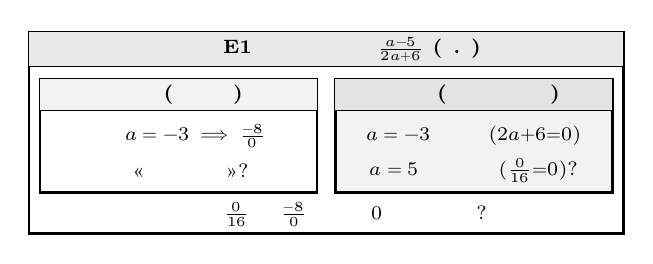
\begin{tikzpicture}[x=1cm, y=1cm, every node/.style={font=\scriptsize, text=black}]
  \draw[black, line width=0.9pt] (0,0) rectangle (7.55,2.56);
  \fill[gray!18] (0,2.12) rectangle (7.55,2.56);
  \draw[black, line width=0.6pt] (0,2.12) -- (7.55,2.12);
  \node at (3.775,2.34) {\textbf{បេសកកម្ម \en{E1}៖ ពិនិត្យកន្សោមសនិទាន $\tfrac{a - 5}{2a + 6}$ (ទំ.៧៦)}};

  % Student A
  \draw[black, line width=0.8pt] (0.14,0.52) rectangle (3.66,1.96);
  \fill[gray!10] (0.14,1.56) rectangle (3.66,1.96);
  \draw[black, line width=0.5pt] (0.14,1.56) -- (3.66,1.56);
  \node at (1.90,1.76) {\textbf{សិស្ស ក (មើលតែភាគបែង)}};
  \node at (1.90,1.24) {ចំពោះ $a = -3 \implies \tfrac{-8}{0}$};
  \node at (1.90,0.80) {ថា៖ «កន្សោម\textbf{ស្មើសូន្យ}»?};

  % Student B
  \draw[black, line width=0.95pt, fill=gray!10] (3.89,0.52) rectangle (7.41,1.96);
  \fill[gray!22] (3.89,1.56) rectangle (7.41,1.96);
  \draw[black, line width=0.55pt] (3.89,1.56) -- (7.41,1.56);
  \node at (5.65,1.76) {\textbf{សិស្ស ខ (ពិនិត្យទាំងពីរផ្នែក)}};
  \node at (5.65,1.24) {$a = -3$ \textbf{គ្មានន័យ} ($2a{+}6{=}0$)};
  \node at (5.65,0.80) {$a = 5$ ទើប\textbf{ស្មើសូន្យ} ($\tfrac{0}{16}{=}0$)?};

  \node at (3.775,0.24) {\textbf{សំណួរ៖} តើ $\tfrac{0}{16}$ និង $\tfrac{-8}{0}$ មួយណាស្មើ $0$ ហើយមួយណាគ្មានន័យ?};
\end{tikzpicture}}

% ២. E2 Explore: ចាត់ថ្នាក់កន្សោមសនិទាន និងតារាងតម្លៃលេខ 3x/(x-2) (ទំ.៧៥--៧៦)
\newcommand{\figExploreRATSixOne}{%
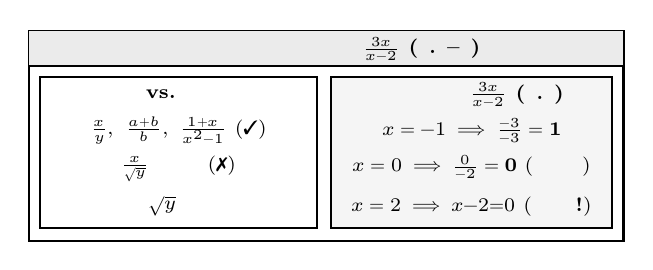
\begin{tikzpicture}[x=1cm, y=1cm, every node/.style={font=\scriptsize, text=black}]
  \draw[black, line width=0.9pt] (0,0) rectangle (7.55,2.66);
  \fill[gray!16] (0,2.22) rectangle (7.55,2.66);
  \draw[black, line width=0.6pt] (0,2.22) -- (7.55,2.22);
  \node at (3.775,2.44) {\textbf{កន្សោមសនិទាន និងការគណនាតម្លៃលេខនៃ $\tfrac{3x}{x-2}$ (ទំ.៧៥--៧៦)}};

  % Left: Rational vs Non-rational
  \draw[black, line width=0.8pt] (0.14,0.16) rectangle (3.66,2.08);
  \node at (1.90,1.86) {\textbf{សនិទាន vs. មិនមែនសនិទាន}};
  \node at (1.90,1.40) {$\tfrac{x}{y},\ \tfrac{a+b}{b},\ \tfrac{1+x}{x^2-1}$ (\ding{51})};
  \node at (1.90,0.92) {$\tfrac{x}{\sqrt{y}}$ \textbf{មិនមែនទេ} (\ding{55})};
  \node at (1.90,0.44) {ព្រោះ $\sqrt{y}$ មិនមែនពហុធា};

  % Right: Evaluation of 3x/(x-2)
  \draw[black, line width=0.8pt, fill=gray!8] (3.84,0.16) rectangle (7.41,2.08);
  \node at (5.625,1.86) {\textbf{ជំនួសតម្លៃក្នុង $\tfrac{3x}{x-2}$ (ទំ.៧៦)}};
  \node at (5.625,1.40) {$x = -1 \implies \tfrac{-3}{-3} = \mathbf{1}$};
  \node at (5.625,0.94) {$x = 0 \implies \tfrac{0}{-2} = \mathbf{0}$ (ស្មើសូន្យ)};
  \node at (5.625,0.44) {$x = 2 \implies x{-}2{=}0$ (\textbf{គ្មានន័យ!})};
\end{tikzpicture}}

% ៣. E3 Explain: លក្ខខណ្ឌទាំង ៣ នៃកន្សោមសនិទាន A/B (ទំ.៧៥--៧៦)
\newcommand{\figRuleRATSixOne}{%
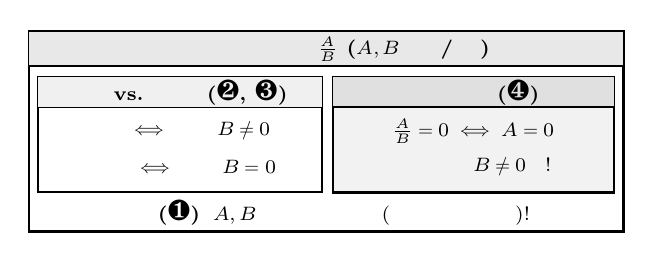
\begin{tikzpicture}[x=1cm, y=1cm, every node/.style={font=\scriptsize, text=black}]
  \draw[black, line width=0.9pt] (0,0) rectangle (7.55,2.54);
  \fill[gray!18] (0,2.10) rectangle (7.55,2.54);
  \draw[black, line width=0.6pt] (0,2.10) -- (7.55,2.10);
  \node at (3.775,2.32) {\textbf{លក្ខខណ្ឌគ្រឹះនៃកន្សោមសនិទាន $\tfrac{A}{B}$ ($A, B$ ជាឯកធា/ពហុធា)}};

  % Left: Meaningful vs Undefined
  \draw[black, line width=0.8pt] (0.12,0.50) rectangle (3.72,1.96);
  \fill[gray!12] (0.12,1.58) rectangle (3.72,1.96);
  \draw[black, line width=0.55pt] (0.12,1.58) -- (3.72,1.58);
  \node at (1.92,1.77) {\textbf{មានន័យ vs. គ្មានន័យ (\cnum{2}, \cnum{3})}};
  \node at (1.92,1.28) {\textbf{មានន័យ} $\iff$ ភាគបែង $B \neq 0$};
  \node at (1.92,0.82) {\textbf{គ្មានន័យ} $\iff$ ភាគបែង $B = 0$};

  % Right: Zero value
  \draw[black, line width=0.95pt, fill=gray!10] (3.86,0.50) rectangle (7.43,1.96);
  \fill[gray!24] (3.86,1.58) rectangle (7.43,1.96);
  \draw[black, line width=0.6pt] (3.86,1.58) -- (7.43,1.58);
  \node at (5.645,1.77) {\textbf{កន្សោមស្មើសូន្យ (\cnum{4})}};
  \node at (5.645,1.28) {$\tfrac{A}{B} = 0 \iff A = 0$};
  \node at (5.645,0.82) {ដោយត្រូវផ្ទៀង $B \neq 0$ ផង!};

  \node at (3.775,0.24) {\textbf{ចំណាំ (\cnum{1})៖} $A, B$ ត្រូវតែជាឯកធា ឬពហុធា (គ្មានអថេរក្រោមរ៉ាឌីកាល់)!};
\end{tikzpicture}}

% ៤. E4 Elaborate: លំហាត់គំរូទំ.៧៥ និងប្រតិបត្តិ 4/(x^2+1) ទំ.៧៦
\newcommand{\figElaborateRATSixOne}{%
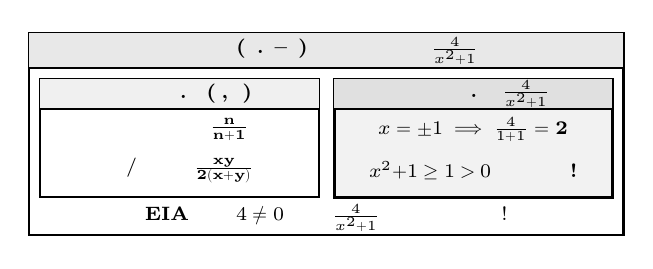
\begin{tikzpicture}[x=1cm, y=1cm, every node/.style={font=\scriptsize, text=black}]
  \draw[black, line width=0.9pt] (0,0) rectangle (7.55,2.56);
  \fill[gray!18] (0,2.12) rectangle (7.55,2.56);
  \draw[black, line width=0.6pt] (0,2.12) -- (7.55,2.12);
  \node at (3.775,2.34) {\textbf{លំហាត់គំរូ (ទំ.៧៥--៧៦)៖ ផលធៀបធរណីមាត្រ និង $\tfrac{4}{x^2+1}$}};

  % Left
  \draw[black, line width=0.8pt] (0.14,0.48) rectangle (3.68,1.98);
  \fill[gray!12] (0.14,1.60) rectangle (3.68,1.98);
  \draw[black, line width=0.55pt] (0.14,1.60) -- (3.68,1.60);
  \node at (1.91,1.79) {\textbf{លំហាត់គំរូ ទំ.៧៥ (ក, ខ)}};
  \node at (1.91,1.34) {ពីរចំនួនគត់តគ្នា៖ $\mathbf{\tfrac{n}{n+1}}$};
  \node at (1.91,0.82) {ផ្ទៃ/បរិមាត្រ៖ $\mathbf{\tfrac{xy}{2(x+y)}}$};

  % Right
  \draw[black, line width=0.95pt, fill=gray!10] (3.88,0.48) rectangle (7.41,1.98);
  \fill[gray!24] (3.88,1.60) rectangle (7.41,1.98);
  \draw[black, line width=0.6pt] (3.88,1.60) -- (7.41,1.60);
  \node at (5.645,1.79) {\textbf{ប្រតិបត្តិ ទំ.៧៦៖ $\tfrac{4}{x^2+1}$}};
  \node at (5.645,1.34) {$x = \pm 1 \implies \tfrac{4}{1+1} = \mathbf{2}$};
  \node at (5.645,0.82) {$x^2{+}1 \ge 1 > 0$ \textbf{មានន័យជានិច្ច!}};

  \node at (3.775,0.22) {\textbf{\en{EIA}៖} ភាគយក $4 \neq 0$ នាំឱ្យ $\tfrac{4}{x^2+1}$ មិនអាចស្មើនឹងសូន្យឡើយ!};
\end{tikzpicture}}

% ៥. E5 Evaluate: ជម្រើសវិនិច្ឆ័យ A-D តម្លៃ x ធ្វើឱ្យ (x-4)/(x+2) គ្មានន័យ
\newcommand{\figExitRATSixOne}{%
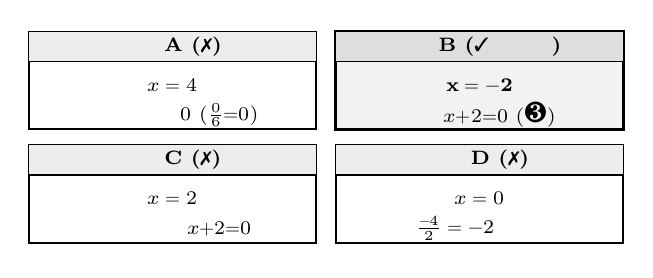
\begin{tikzpicture}[x=1cm, y=1cm, every node/.style={font=\scriptsize, text=black}]
  % Choice A
  \draw[black, line width=0.8pt] (0,1.44) rectangle (3.65,2.68);
  \fill[gray!14] (0,2.30) rectangle (3.65,2.68);
  \draw[black, line width=0.5pt] (0,2.30) -- (3.65,2.30);
  \node at (1.825,2.49) {\textbf{ជម្រើស \en{A} (\ding{55})}};
  \node at (1.825,2.00) {$x = 4$};
  \node at (1.825,1.62) {ធ្វើឱ្យភាគយកស្មើ $0$ ($\tfrac{0}{6}{=}0$)};

  % Choice B (Correct)
  \draw[black, line width=1.0pt, fill=gray!10] (3.90,1.44) rectangle (7.55,2.68);
  \fill[gray!26] (3.90,2.30) rectangle (7.55,2.68);
  \draw[black, line width=0.55pt] (3.90,2.30) -- (7.55,2.30);
  \node at (5.725,2.49) {\textbf{ជម្រើស \en{B} (\ding{51} ត្រឹមត្រូវ)}};
  \node at (5.725,2.00) {$\mathbf{x = -2}$};
  \node at (5.725,1.62) {ភាគបែង $x{+}2{=}0$ (\cnum{3})};

  % Choice C
  \draw[black, line width=0.8pt] (0,0) rectangle (3.65,1.24);
  \fill[gray!14] (0,0.86) rectangle (3.65,1.24);
  \draw[black, line width=0.5pt] (0,0.86) -- (3.65,0.86);
  \node at (1.825,1.05) {\textbf{ជម្រើស \en{C} (\ding{55})}};
  \node at (1.825,0.56) {$x = 2$};
  \node at (1.825,0.18) {ច្រឡំសញ្ញាពេលដោះ $x{+}2{=}0$};

  % Choice D
  \draw[black, line width=0.8pt] (3.90,0) rectangle (7.55,1.24);
  \fill[gray!14] (3.90,0.86) rectangle (7.55,1.24);
  \draw[black, line width=0.5pt] (3.90,0.86) -- (7.55,0.86);
  \node at (5.725,1.05) {\textbf{ជម្រើស \en{D} (\ding{55})}};
  \node at (5.725,0.56) {$x = 0$};
  \node at (5.725,0.18) {បាន $\tfrac{-4}{2} = -2$ មានន័យធម្មតា};
\end{tikzpicture}}

% ============================================================================
% ៦. ចាប់ផ្ដើមឯកសារ (Document Body)
% ============================================================================
\begin{document}
\fontsize{10pt}{15.2pt}\selectfont

% --- ក្បាលរដ្ឋបាល (Administrative Header) ---
\begin{center}
  {\muol\fontsize{11pt}{16pt}\selectfont ព្រះរាជាណាចក្រកម្ពុជា}\\[2pt]
  {\muol\fontsize{11pt}{16pt}\selectfont ជាតិ សាសនា ព្រះមហាក្សត្រ}\\[-2pt]
  \khmflourish
\end{center}
\vspace{-4pt}

{\muol\fontsize{10pt}{15pt}\selectfont
មន្ទីរអប់រំ យុវជន និងកីឡា ខេត្តកំពង់ធំ\\
ការិយាល័យអប់រំ យុវជន និងកីឡា ស្រុកកំពង់ស្វាយ\\
អនុវិទ្យាល័យព្រះក្រសាំង}

\vspace{2pt}
\begin{center}
  {\muol\fontsize{12pt}{18pt}\selectfont កិច្ចតែងការបង្រៀន}
\end{center}
\vspace{1pt}

% --- ព័ត៌មានទូទៅ (General Metadata) ---
\begin{tabular}{@{}p{1.85cm}p{3.25cm}@{\hspace{4pt}:\hspace{6pt}}p{12.65cm}@{}}
  & - \quad មុខវិជ្ជា          & គណិតវិទ្យា ថ្នាក់ទី៨ (ពីជគណិត) \\
  & - \quad ចំណងជើងមេរៀន & មេរៀនទី៦៖ កន្សោមសនិទាន \\
  & - \quad ចំណងជើងរង      & ១. កន្សោមសនិទាន និង ២. តម្លៃលេខនៃកន្សោមសនិទាន \\
  & - \quad រយៈពេល             & ១ ម៉ោងសិក្សា (៥០ នាទី) \\
  & - \quad បង្រៀនដោយ         & ហុក ប៊ុនថែន \\
  & - \quad កាលបរិច្ឆេទ        & ថ្ងៃចន្ទ ទី១៤ ខែធ្នូ ឆ្នាំ២០២៦ \\
\end{tabular}

\vspace{4pt}

% --- I. វត្ថុបំណង ---
{\muol\enbf{I.} វត្ថុបំណង}\par\vspace{2pt}
\begin{tabular}{@{}p{0.55cm}p{2.55cm}@{\hspace{2pt}:\hspace{6pt}}L{15.4cm}@{}}
  & \wcirc វិជ្ជាសម្បទា   & សិស្សប្រាប់បាននូវនិយមន័យកន្សោមសនិទាន $\tfrac{A}{B}$ ($B \neq 0$) ព្រមទាំងលក្ខខណ្ឌដែលកន្សោមសនិទានមានន័យ គ្មានន័យ និងស្មើនឹងសូន្យបានត្រឹមត្រូវ (ទំ.៧៥–៧៦) ។ \\[2pt]
  & \wcirc បំណិនសម្បទា & សិស្សសរសេរផលធៀបជាកន្សោមសនិទាន គណនាតម្លៃលេខ និងរកតម្លៃអថេរធ្វើឱ្យកន្សោមមានន័យ គ្មានន័យ ឬស្មើសូន្យលើសន្លឹកកិច្ចការបានត្រឹមត្រូវ ។ \\[2pt]
  & \wcirc ចរិយាសម្បទា  & សិស្សមានទម្លាប់ត្រួតពិនិត្យលក្ខខណ្ឌភាគបែងខុសពីសូន្យ ($B \neq 0$) ជានិច្ចមុនគណនាតម្លៃលេខប្រកបដោយភាពហ្មត់ចត់ ។ \\
\end{tabular}

\vspace{3pt}

% --- II. សម្ភារៈឧបទេស (Zero-LCD & Fill-In Worksheet Context) ---
{\muol\enbf{II.} សម្ភារៈឧបទេស}\par\vspace{2pt}
\hspace*{0.55cm}$\bullet$ សៀវភៅសិក្សាគោលថ្នាក់ទី៨ (ទំ.៧៥--៧៦, ៨៥) ក្ដារខៀន ដីស/ហ្វឺត បន្ទាត់ត្រង់ និង\textbf{សន្លឹកកិច្ចការសិស្សបំពេញចន្លោះ ស-ខ្មៅ} (កូដ \en{RAT61} ទំព័រ ១--២ សម្រាប់សិស្ស និងទំព័រ ៣ ប្លង់ក្ដារខៀន/ចម្លើយគ្រូ — គ្មានប្រើ \en{LCD})

\vspace{3pt}

% --- III. វិធីសាស្រ្តបង្រៀន ---
{\muol\enbf{III.} វិធីសាស្រ្តបង្រៀន}\par\vspace{2pt}
\begin{tabular}{@{}p{0.55cm}p{2.55cm}@{\hspace{2pt}:\hspace{6pt}}L{15.4cm}@{}}
  & $\bullet$ គោលវិធី      & សិស្សមជ្ឈមណ្ឌល (សន្លឹកកិច្ចការបំពេញចន្លោះជាគោល + ការពិភាក្សាជាក្រុមតូច ៣ នាក់) \\
  & $\bullet$ យុទ្ធវិធីបង្រៀន & គំរូស្ថាបនានិយម \en{5Es} រួមបញ្ចូល \textit{ការប្រៀបធៀបករណីផ្ទុយនៃលេខសូន្យ (\en{Contrasting Zero Cases})} និង \textit{ការតេស្តតម្លៃព្រំដែន} \\
\end{tabular}

\vspace{4pt}

% --- IV. ដំណើរការបង្រៀន (50-Minute 5E Flow) ---
{\muol\enbf{IV.} ដំណើរការបង្រៀន}\par\vspace{1pt}

\renewcommand{\arraystretch}{1.15}
\begin{longtable}{|L{5.50cm}|L{7.90cm}|L{4.80cm}|}
\hline
\multicolumn{1}{|c|}{\cellcolor{headgray}\muol សកម្មភាពគ្រូ} &
\multicolumn{1}{c|}{\cellcolor{headgray}\muol ខ្លឹមសារមេរៀន} &
\multicolumn{1}{c|}{\cellcolor{headgray}\muol សកម្មភាពសិស្ស} \\[2pt]
\hline
\endfirsthead

\hline
\multicolumn{1}{|c|}{\cellcolor{headgray}\muol សកម្មភាពគ្រូ} &
\multicolumn{1}{c|}{\cellcolor{headgray}\muol ខ្លឹមសារមេរៀន} &
\multicolumn{1}{c|}{\cellcolor{headgray}\muol សកម្មភាពសិស្ស} \\[2pt]
\hline
\endhead

\hline
\endfoot

% ==================== ជំហានទី១ (2min) ====================
\stepheader{ជំហានទី១ \enbf{(}រដ្ឋបាលថ្នាក់\enbf{)}}
$\bullet$ ពិនិត្យវត្តមាន អនាម័យ និងសណ្ដាប់ធ្នាប់ថ្នាក់រៀន \par
$\bullet$ រៀបចំក្រុមតូច ៣ នាក់ និងចែក\textbf{សន្លឹកកិច្ចការសិស្ស} (\en{RAT61} ទំព័រ ១–២)
&
$\bullet$ រដ្ឋបាលថ្នាក់ អនាម័យ និងវិន័យសិក្សា \par
$\bullet$ ចែកសន្លឹកកិច្ចការម្នាក់ ១ សន្លឹក សម្រាប់បំពេញតាមដំណាក់កាល \en{E1--E5}
&
$\circ$ ប្រធានថ្នាក់រាយការណ៍វត្តមានសិស្ស \par
$\circ$ ទទួលសន្លឹកកិច្ចការ សរសេរឈ្មោះ និងអង្គុយតាមក្រុម ៣ នាក់ \\
\hline

% ==================== ជំហានទី២ (9min: កំណែ ≤3m + រំលឹក 3m + E1 3m) ====================
\stepheader{ជំហានទី២ \enbf{(}កិច្ចការផ្ទះ \enbf{+} ទំនាក់ទំនងមេរៀនថ្មី\enbf{)}}
\ditem \textbf{កំណែកិច្ចការផ្ទះមេរៀនទី៥ (\enbf{$\le$ 3 min})} \par
$\bullet$ ហៅសិស្ស ២ នាក់ឡើងកែលំហាត់ទំ.៧៤ \en{\#12} ង និង \en{\#15} ឃ, ង លើក្ដារខៀន
&
\hspace*{0.15cm}\redsub{កំណែកិច្ចការផ្ទះ (បញ្ចប់មេរៀនទី៥ ទំ.៧៤)} \par
$\bullet$ \textbf{\en{\#12} ង និង \en{\#16} គ ($C$)៖} $(y-8)(5y-1)$; \quad $(2x-3)(2x-1)$ \par
$\bullet$ \textbf{\en{\#15} ឃ, ង, ជ៖} $(2x+1)(x+7)$; \quad $2(7a-5)(a+2)$; \quad $(2x+1)(3x+1)$
&
$\circ$ ផ្ទៀងចម្លើយ និងកែតម្រូវចូលសៀវភៅកិច្ចការផ្ទះ \\[3pt]

\ditem \textbf{រំលឹកមេរៀនទាក់ទង (\enbf{3min})} \par
$\bullet$ សួរ៖ «ក្នុងចំនួនសនិទាន $\tfrac{p}{q}$ ($p, q \in \mathbb{Z}$) តើ $q$ អាចស្មើនឹង $0$ បានឬទេ? ចុះ $\tfrac{0}{5}$ និង $\tfrac{5}{0}$ ខុសគ្នាដូចម្ដេច?»
&
\hspace*{0.15cm}\redsub{រំលឹកចំនួនសនិទាន និងការចែកនឹងសូន្យ} \par
$\bullet$ ចំនួនសនិទាន $\dfrac{p}{q}$ មានន័យលុះត្រាតែភាគបែង $q \neq 0$ \par
$\bullet$ $\dfrac{0}{5} = 0$ (ព្រោះ $0 = 5 \times 0$) ឯ $\dfrac{5}{0}$ \textbf{គ្មានន័យ} (ចែកនឹង $0$ មិនបានទេ!)
&
$\circ$ ឆ្លើយ៖ «$q \neq 0$! $\tfrac{0}{5} = 0$ ឯ $\tfrac{5}{0}$ គ្មានន័យ!» \\[3pt]

\fiveE{E1 - Engage (3min)} \timenote{(កុំទាន់ផ្តល់ចម្លើយ)} \par
\ditem \textbf{បេសកកម្មអន្ទាក់តួនាទីលេខសូន្យ (សន្លឹកកិច្ចការ \en{E1})} \par
$\bullet$ ឱ្យសិស្សអានប្រអប់ \en{E1} ពិនិត្យកន្សោម $\dfrac{a - 5}{2a + 6}$ (ទំ.៧៦) រវាងសិស្ស ក និងសិស្ស ខ
&
\redsub{បេសកកម្ម \en{E1}៖ ស្មើសូន្យ ឬគ្មានន័យក្នុង $\dfrac{a - 5}{2a + 6}$? (ទំ.៧៦)} \par
$\bullet$ \textbf{សិស្ស ក} ថា៖ «ពេល $a = -3$ ភាគបែងស្មើ $0$ ដូចនេះកន្សោមស្មើសូន្យ»! \par
$\bullet$ \textbf{សិស្ស ខ} ថា៖ «ពេល $a = -3$ កន្សោមគ្មានន័យ ឯស្មើសូន្យគឺពេល $a = 5$»!
&
$\circ$ ជំនួស $a = -3$ និង $a = 5$ ពិភាក្សាជាគូ និងគូស \ding{51} លើ \en{E1} \\[3pt]

&
\cfig{\figEngageRATSixOne}
& \\
\hline

% ==================== ជំហានទី៣ (17min: E2 11m + E3 6m) ====================
\stepheader{ជំហានទី៣ \enbf{(}ខ្លឹមសារមេរៀនថ្មី\enbf{)}}
\fiveE{E2 - Explore (11min)} \par
$\bullet$ សរសេរចំណងជើង \textbf{មេរៀនទី៦៖ កន្សោមសនិទាន (១–២)} លើក្ដារខៀន \par
\ditem \textbf{សកម្មភាព ១៖ ស្គាល់កន្សោមសនិទាន vs. មិនមែនសនិទាន (ទំ.៧៥, \enbf{5min}, \en{E2-A})} \par
$\bullet$ ឱ្យសិស្សពិនិត្យភាគយកនិងភាគបែងនៃកន្សោមក្នុងឧទាហរណ៍ទំ.៧៥ លើ \en{E2-A}
&
១. កន្សោមសនិទាន (ទំ.៧៥) \par
$\bullet$ $\dfrac{x}{y}$, $\dfrac{a+b}{b}$ និង $\dfrac{1+x}{x^2-1}$ មានភាគយកនិងភាគបែងជាឯកធា ឬពហុធា $\implies$ ហៅថា \textbf{កន្សោមសនិទាន} \par
$\bullet$ \textbf{សម្គាល់៖} $\dfrac{x}{\sqrt{y}}$ \textbf{ពុំមែន}ជាកន្សោមសនិទានទេ ព្រោះ $\sqrt{y}$ ពុំមែនជាឯកធា ឬពហុធាឡើយ
&
$\circ$ ចាត់ថ្នាក់កន្សោមសនិទាន និងពន្យល់មូលហេតុលើ \en{E2-A} \\[3pt]

\ditem \textbf{សកម្មភាព ២៖ គណនាតម្លៃលេខនៃ $\dfrac{3x}{x - 2}$ (ទំ.៧៦, \enbf{6min}, \en{E2-B})} \par
$\bullet$ ឱ្យសិស្សជំនួស $x = -1$, $x = 0$ និង $x = 2$ ចូលក្នុង $\dfrac{3x}{x - 2}$ លើ \en{E2-B}
&
២. តម្លៃលេខនៃកន្សោមសនិទាន (ទំ.៧៦) \par
$\bullet$ ចំពោះ $x = -1$៖ $\dfrac{3(-1)}{-1 - 2} = \dfrac{-3}{-3} = \mathbf{1}$;\quad ចំពោះ $x = 0$៖ $\dfrac{3\times 0}{0 - 2} = \dfrac{0}{-2} = \mathbf{0}$ \par
$\bullet$ ចំពោះ $x = 2$៖ ភាគបែង $x - 2 = 2 - 2 = 0$ ក្នុងករណីនេះ \textbf{កន្សោមគ្មានន័យ}!
&
$\circ$ ជំនួសតម្លៃទាំង ៣ និងសង្កេតករណី $x = 2$ លើ \en{E2-B} \\[3pt]

&
\cfig{\figExploreRATSixOne}
& \\[3pt]

% --- E3 Explain (6min) ---
\fiveE{E3 - Explain (6min)} \par
$\bullet$ ដឹកនាំសិស្សទាញនិយមន័យ និងលក្ខខណ្ឌទាំង ៣ នៃកន្សោមសនិទាន (ទំ.៧៥–៧៦)
&
$\bullet$ \textbf{ជាទូទៅ (ទំ.៧៥–៧៦)៖} \par
\hspace*{0.15cm}– \textbf{កន្សោមសនិទាន} មានទម្រង់ $\graybox{$\dfrac{A}{B}$}$ ដែល $A, B$ ជាឯកធា ឬពហុធា ($B \neq 0$) \par
\hspace*{0.15cm}– \textbf{មានន័យ} $\iff \graybox{$B \neq 0$}$;\quad \textbf{គ្មានន័យ} $\iff B = 0$;\quad \textbf{ស្មើសូន្យ} $\iff \graybox{$A = 0\text{ និង }B \neq 0$}$
&
$\circ$ បំពេញប្រអប់និយមន័យ និងលក្ខខណ្ឌទាំង ៣ លើ \en{E3} \\[3pt]

$\bullet$ ភ្ជាប់\textbf{ធនាគារហេតុផល \cnum{1}--\cnum{4}} លើក្ដារខៀន និងសន្លឹកកិច្ចការ
&
\textbf{ធនាគារហេតុផល (\en{Warrant Bank})៖} \par
\cnum{1} \textbf{លក្ខណៈពហុធា៖} ភាគយក $A$ និងភាគបែង $B$ ត្រូវជាឯកធា ឬពហុធា (គ្មានអថេរក្រោម $\sqrt{\phantom{x}}$) \par
\cnum{2} \textbf{លក្ខខណ្ឌមានន័យ៖} កន្សោមសនិទានមានន័យលុះត្រាតែភាគបែងខុសពីសូន្យ ($B \neq 0$)
&
$\circ$ ផ្ទៀងលេខកូដ \cnum{1}--\cnum{2} លើសន្លឹកកិច្ចការ \\[3pt]

&
\cnum{3} \textbf{លក្ខខណ្ឌគ្មានន័យ៖} កន្សោមសនិទានគ្មានន័យកាលណាភាគបែងស្មើនឹងសូន្យ ($B = 0$)
&
$\circ$ ផ្ទៀងលេខកូដ \cnum{3} លើសន្លឹកកិច្ចការ \\[3pt]

&
\cnum{4} \textbf{លក្ខខណ្ឌស្មើសូន្យ៖} $\tfrac{A}{B} = 0$ លុះត្រាតែភាគយក $A = 0$ ហើយភាគបែង $B \neq 0$ ក្នុងពេលតែមួយ
&
$\circ$ ផ្ទៀងលេខកូដ \cnum{4} លើសន្លឹកកិច្ចការ \\[3pt]

&
\cfig{\figRuleRATSixOne}
& \\
\hline

% ==================== ជំហានទី៤ (20min: E4 10m + E5 10m) ====================
\stepheader{ជំហានទី៤ \enbf{(}ពង្រីកចំណេះដឹង\enbf{)}}
\fiveE{E4 - Elaborate (10min)} \par
\ditem \textbf{លំហាត់គំរូ៖ បង្កើតកន្សោមសនិទាន និងសិក្សា $\dfrac{4}{x^2+1}$ (ទំ.៧៥–៧៦)} \par
$\bullet$ ឱ្យសិស្សធ្វើលំហាត់គំរូទំ.៧៥ (ក, ខ) លំហាត់គំរូទំ.៧៦ និងប្រតិបត្តិទំ.៧៦ លើ \en{E4}
&
\textbf{លំហាត់គំរូពង្រីក (ទំ.៧៥–៧៦)៖} \par
$\bullet$ \textbf{១) លំហាត់គំរូ ទំ.៧៥៖} ក) ពីរចំនួនគត់តគ្នា $\to \mathbf{\dfrac{n}{n+1}}$;\quad ខ) ផ្ទៃធៀបបរិមាត្រចតុកោណកែង $\to \graybox{$\dfrac{xy}{2(x+y)}$}$ \par
$\bullet$ \textbf{២) លំហាត់គំរូ ទំ.៧៦ ($\dfrac{a-5}{2a+6}$)៖} ក) គ្មានន័យ $\iff 2a+6=0 \implies \mathbf{a = -3}$;\quad ខ) ស្មើសូន្យ $\implies \mathbf{a = 5}$ \par
$\bullet$ \textbf{៣) ប្រតិបត្តិ ទំ.៧៦ ($\dfrac{4}{x^2+1}$)៖} ចំពោះ $x = \pm 1$ បាន $\dfrac{4}{2} = \mathbf{2}$ \par
\hspace*{0.15cm}– ព្រោះភាគយក $4 \neq 0$ និងភាគបែង $x^2 + 1 \ge 1 > 0$ នាំឱ្យកន្សោមមានន័យជានិច្ច និងមិនអាចស្មើសូន្យឡើយ!
&
$\circ$ បង្កើតកន្សោម និងវិភាគករណី $x^2+1 \ge 1$ លើ \en{E4} \\[3pt]

&
\cfig{\figElaborateRATSixOne}
& \\[3pt]

$\bullet$ សួរសំណួរឆ្លុះបញ្ចាំង \textbf{\en{EIA Looking-Back}} (\enbf{1min})
&
\textbf{\en{EIA Looking-Back}៖} «ហេតុអ្វីកន្សោម $\dfrac{4}{x^2 + 1}$ គ្មានតម្លៃ $x \in \mathbb{R}$ ណាមួយធ្វើឱ្យវាគ្មានន័យសោះ?» ($\to$ ព្រោះ $x^2 \ge 0 \implies x^2 + 1 \ge 1 > 0$ ខុសពីសូន្យជានិច្ច \cnum{2}!)
&
$\circ$ ពន្យល់ដោយសម្គាល់ថា $x^2 + 1 \ge 1$ គ្រប់ចំនួនពិត $x$ \\[3pt]

% --- E5 Evaluate (10min) ---
\fiveE{E5 - Evaluate (10min)} \par
\ditem \textbf{ប្រតិបត្តិជាក្រុមតូច ៣ នាក់ (\enbf{4min}, សន្លឹកកិច្ចការ \en{E5})} \par
$\bullet$ ឱ្យសិស្សដោះស្រាយប្រតិបត្តិទំ.៧៥ និងលំហាត់ទំ.៨៥ (\en{\#2} ក, គ, \en{\#3} ក, \en{\#4} ក)
&
\textbf{លំហាត់ប្រតិបត្តិ (ទំ.៧៥ និង ទំ.៨៥ \en{\#2, \#3, \#4})៖} \par
$\bullet$ \textbf{១) ប្រតិបត្តិ ទំ.៧៥ និង \en{\#2} ក៖} ផ្ទៃរង្វង់ធៀបការេ $\graybox{$\dfrac{\pi r^2}{x^2}$}$; \quad $\dfrac{7x}{6x+7}$ មានន័យពេល $\mathbf{x \neq -\dfrac{7}{6}}$ \par
$\bullet$ \textbf{២) \en{\#2} គ, \en{\#3} ក និង \en{\#4} ក៖} \en{\#2} គ) $\mathbf{x \neq -4,\ 3}$; \quad \en{\#3} ក) គ្មានន័យពេល $\mathbf{a = 1}$; \quad \en{\#4} ក) ស្មើសូន្យពេល $\mathbf{x = \dfrac{3}{2}}$
&
$\circ$ សហការគ្នាដោះស្រាយលើ \en{E5} បានត្រឹមត្រូវ \\[3pt]

$\bullet$ ឱ្យក្រុមសិស្សផ្ទៀងផ្ទាត់និងបិទ\textbf{បេសកកម្ម \en{E1}} (\enbf{2min})
&
$\bullet$ \textbf{បិទបេសកកម្ម \en{E1}៖} សិស្ស ខ ត្រឹមត្រូវ! ចំពោះ $a = -3$ បានភាគបែង $0$ (\textbf{គ្មានន័យ}) ឯស្មើសូន្យគឺពេល $a = 5$ (\ding{51})!
&
$\circ$ បិទបេសកកម្ម \en{E1} ឃើញសិស្ស ខ ត្រឹមត្រូវ \\[3pt]

\ditem \textbf{សំណួរវិនិច្ឆ័យ \en{A--D} និងសំបុត្រចេញ (\enbf{4min})} \par
$\bullet$ ឱ្យសិស្សគូសរង្វង់ជម្រើសត្រូវលើសន្លឹកកិច្ចការ រួចលើកម្រាមដៃ ១--៤
&
\centering\textbf{សំណួរវិនិច្ឆ័យ \en{A--D}៖ តើតម្លៃ $x$ ណាដែលធ្វើឱ្យ $\dfrac{x - 4}{x + 2}$ គ្មានន័យ?}\par
\textbf{\en{A.}} $x = 4$ \qquad
\textbf{\en{B.}} $x = -2$ \qquad
\textbf{\en{C.}} $x = 2$ \qquad
\textbf{\en{D.}} $x = 0$\par
{\itshape (កត់សម្គាល់៖ កន្សោមសនិទានគ្មានន័យកាលណាភាគបែងស្មើនឹងសូន្យ)}
&
$\circ$ គិតរហ័ស និងលើកម្រាមដៃ ២ (\textbf{ជម្រើស \en{B}៖} $x = -2$) \\[3pt]

&
\cfig{\figExitRATSixOne}
& \\[3pt]

$\bullet$ បញ្ជាក់ចម្លើយត្រូវ (\textbf{ជម្រើស \en{B}}) និងឱ្យបំពេញសំបុត្រចេញ ៦០ វិនាទី
&
$\bullet$ \textbf{សំបុត្រចេញ (ទំ.៨៥ \en{\#2} ខ)៖} កន្សោមសនិទាន $\dfrac{3x}{(x - 3)^2}$ មានន័យលុះត្រាតែ $(x-3)^2 \neq 0 \iff \mathbf{x \neq 3}$ ។
&
$\circ$ បំពេញសំបុត្រចេញលើសន្លឹកកិច្ចការមុនបញ្ចប់ម៉ោង \\
\hline

% ==================== ជំហានទី៥ (≤2min) ====================
\stepheader{ជំហានទី៥ \enbf{(}កិច្ចការផ្ទះ \enbf{+} បណ្ដាំផ្ញើ\enbf{)}}
\timenote{ចំណាយពេលឱ្យតិចបំផុតកុំឱ្យលើស 2min} \par
$\bullet$ ណែនាំប្រអប់កិច្ចការផ្ទះលើសន្លឹកកិច្ចការទំព័រ ២ (ទំ.៨៥ \en{\#1, \#2, \#3, \#4})
&
\centering\textbf{កិច្ចការផ្ទះ (សៀវភៅគោល ទំ.៨៥ លេខ ១, ២, ៣, ៤)}\par\raggedright
$\bullet$ \textbf{១) ទំ.៨៥ \en{\#1} ខ៖} គណនាតម្លៃលេខនៃ $\dfrac{-a^2 + 4}{2a^2 - a - 1}$ ចំពោះ $a = -2$, $a = -\dfrac{1}{2}$ និង $a = 1$ ។ \par
$\bullet$ \textbf{២) ទំ.៨៥ \en{\#2} ឃ, \en{\#3} គ និង \en{\#4} គ៖} រកតម្លៃអថេរធ្វើឱ្យ \en{\#2} ឃ មានន័យ, \en{\#3} គ គ្មានន័យ និង \en{\#4} គ ស្មើសូន្យ ។
&
$\circ$ គូសចំណាំកិច្ចការផ្ទះលើសន្លឹកកិច្ចការ \\[3pt]

$\bullet$ ផ្តាំផ្ញើឱ្យអានមុនចំណុច \textbf{៣. ការសម្រួលកន្សោមសនិទាន} (ទំ.៧៦–៧៨)
&
$\bullet$ \textbf{បណ្ដាំផ្ញើ៖} ធ្វើកិច្ចការផ្ទះឱ្យបានគ្រប់គ្នា និងអានមុនចំណុចទី៣ (ការសម្រួលកន្សោមសនិទាន ទំ.៧៦–៧៨) ។
&
$\circ$ កត់ត្រាបណ្ដាំផ្ញើ ទុកសន្លឹកកិច្ចការក្នុងសៀវភៅ និងជម្រាបលាគ្រូ \\
\hline
\end{longtable}

\vspace{6pt}

% --- ហត្ថលេខា (Signature Block) ---
\begin{flushright}
  \begin{minipage}{8.6cm}
    \centering
    ថ្ងៃចន្ទ ៥កើត ខែមិគសិរ ឆ្នាំមមី អដ្ឋស័ក ពុទ្ធសករាជ ២៥៧០\\
    កំពង់ស្វាយ, ថ្ងៃទី១៤ ខែធ្នូ ឆ្នាំ២០២៦\\[4pt]
    {\muol គ្រូបង្រៀន}\\[32pt]
    \hfill{\muol ហុក ប៊ុនថែន}\hspace*{1.4cm}
  \end{minipage}
\end{flushright}

\end{document}
